\documentclass[a4paper]{article}
\usepackage{titling}
\usepackage{authblk}
\usepackage{fancyhdr}
\usepackage[hyphens]{url}
\usepackage{hyperref}
\usepackage{rsc}
\usepackage{siunitx}
\usepackage{graphicx}
\usepackage{mhchem}
\usepackage{amsmath}
\usepackage{listings}
\usepackage{color}
\usepackage[htt]{hyphenat}
\usepackage{subcaption}

\definecolor{dkgreen}{rgb}{0,0.6,0}
\definecolor{gray}{rgb}{0.5,0.5,0.5}
\definecolor{mauve}{rgb}{0.58,0,0.82}


\lstset{frame=tb,
  language=Python,
  aboveskip=3mm,
  belowskip=3mm,
  showstringspaces=false,
  columns=flexible,
  basicstyle={\ttfamily},
  numbers=none,
  numberstyle=\tiny\color{gray},
  keywordstyle=\color{blue},
  commentstyle=\color{dkgreen},
  stringstyle=\color{mauve},
  breaklines=true,
  breakatwhitespace=true,
  tabsize=3,
  postbreak=\mbox{\textcolor{red}{$\hookrightarrow$}\space}
}

\title{Lecture 8: Working with vectors and matrices}
\author[1]{Dr Benjamin J. Morgan}
\author[1,2]{Dr Andrew R. McCluskey}
\affil[1]{Department of Chemistry, University of Bath, email: b.j.morgan@bath.ac.uk}
\affil[2]{Diamond Light Source, email: andrew.mccluskey@diamond.ac.uk}
\setcounter{Maxaffil}{0}
\renewcommand\Affilfont{\itshape\small}

\pagestyle{fancy}
\fancyhf{}
\rhead{CH40208}
\lhead{\thetitle}
\rfoot{\thepage}

\begin{document}
\maketitle

\section*{Aim}
This week gives a brief introduction to \emph{vectors} and \emph{matrices} and using these to perform mathematical manipulations in Python.

\section{Vectors}
Many problems in chemistry and physics involve working with \emph{vector} quantities. A common definition of a vector in a physics context is a quantity with both \emph{magnitude} and \emph{direction}; for example, the positions or velocities of atoms, or the forces acting on atoms within a molecule.

\subsection{Example 1: Atomic positions}
Positions of atoms are always relative, i.e.\ defined with respect to some \emph{origin}.
\begin{figure*}
  \centering
  \begin{subfigure}[b]{0.475\textwidth}
    \centering
    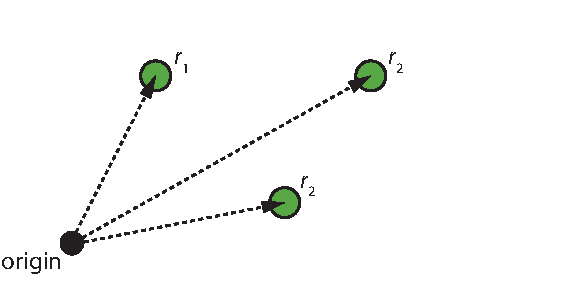
\includegraphics[width=\textwidth]{../figures/position_vectors_1}
    \caption[Network2]%
      {{\small Network 1}}    
    \label{fig:mean and std of net14}
  \end{subfigure}
  \hfill
  \begin{subfigure}[b]{0.475\textwidth}  
    \centering 
    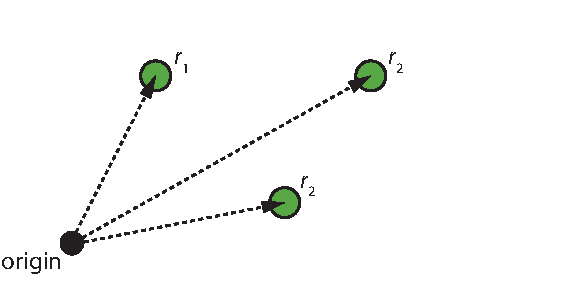
\includegraphics[width=\textwidth]{../figures/position_vectors_1}
    \caption[]%
      {{\small Network 2}}    
    \label{fig:mean and std of net24}
  \end{subfigure}
  \vskip\baselineskip
  \begin{subfigure}[b]{0.475\textwidth}   
    \centering 
    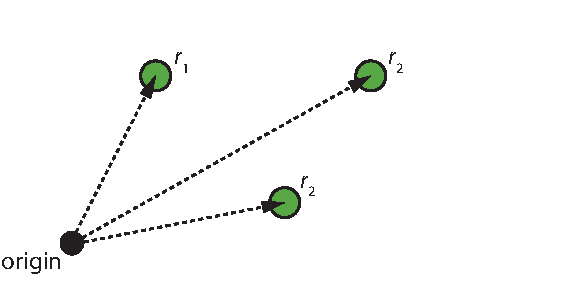
\includegraphics[width=\textwidth]{../figures/position_vectors_1}
    \caption[]%
      {{\small Network 3}}    
    \label{fig:mean and std of net34}
  \end{subfigure}
  \quad
  \begin{subfigure}[b]{0.475\textwidth}   
     \centering 
     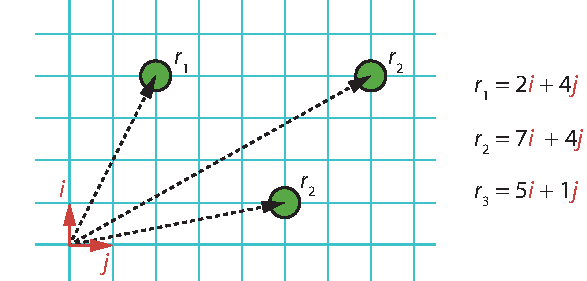
\includegraphics[width=\textwidth]{../figures/position_vectors_4}
     \caption[]%
       {{\small Network 4}}    
     \label{fig:mean and std of net44}
   \end{subfigure}
 \caption[ The average and standard deviation of critical parameters ]
   {\small The average and standard deviation of critical parameters: Region R4} 
 \label{fig:mean and std of nets}
\end{figure*}

One of the benefits of using Python over other programming languages is the clear syntax.
However, we can improve the readablity and comprehensibility of our code further by \emph{writing readable code}.
Now, this isn't a comment on handwriting or grammar but rather a discussion into aspects such as:
\begin{itemize}
  \item{Using sensible variable names}
  \item{Using relevant comments}
  \item{Including descriptive docstrings for functions}
  \item{Attempt to keep line length relatively short}
  \item{Write modular code by writing short functions that perform just a single task and combining with other functions}
\end{itemize}
If we consider the following example, where we are trying to determine which elements in the list below are liquid at room temperature.
The code below is not readable (at least not easily) but it is trying to print the elements that are liquid at room temperature,
\begin{lstlisting}
# Ugly, hard to read code

s = ['H', 'Ca', 'Fe', 'Hg', 'Br', 'Xe']
m = [13.99, 1115, 1811, 234.321, 265.8, 161.4]
b = [20.271, 1757, 3134, 629.88, 332, 165.051]
for d in range(0, len(s)):
    if m[d] < 273.15 and b[d] >= 273.15:
        print(s[d])
        print("This element is a liquid and not a solid or a gas at standard temperature and pressure.")
\end{lstlisting}
It is not immediately clear what this code is aiming to achieve.
For example, the three lists are simply given the names \texttt{s}, \texttt{m}, and \texttt{b}, which the author (currently) knows are short for chemical \texttt{s}ymbols, \texttt{m}elting point, and \texttt{b}oiling point.
However, if someone else was to try and understand this it is not clear, or if the original author comes back to the code many months (or years) later.
There are no comments or documentation to explain the purpose of this code, in particular the \texttt{if} statement would benefit from some rationalisation.
Finally, the final line is very long, running to over 100 characters (when is widely considered that the maximum readbility is found when there is less than 80 characters per line).

\vspace{\baselineskip}
\begin{center}
	\noindent\fbox{%
	    \begin{minipage}{0.9\textwidth}%
	        \vspace{0.15\baselineskip}
			\subsubsection*{Exercise}
	        Rewrite the code to be more readable and clear, remembering to have descriptive variable names, to be concise and to consider iteration conventions.
	    \end{minipage}
	}
\end{center}

\section{Comments and docstrings}
One of the easiest ways to make it more clear what your code is trying to do is to add comments.
These are lines in the code that are ignored by the Python interpreter.
You will have seen these in most of the code blocks in these handouts, where the line starts with a \texttt{\#} symbol.
This means that the line will be ignored, and these can be a great way to give the reason for a particular decision in your code.
For example, before the fifth line of the code block above the following comment could be included,
\begin{lstlisting}
# This line determines if room temperature is between the
# melting and boiling point of the given element
\end{lstlisting}
A comment like this makes the purpose of the \texttt{if} statement much clearer.

A subset of the comments are \emph{docstrings}, these are comments that describe the purpose of a function, often including the expected parameters.
There are a variety of styles that are used in docstrings; the most common are Sphinx, Google, and NumPy.
However, we will focus on using the Google style as it is the most human readable, however you should be aware that these other styles exist.
An example of a docstring is shown in the function definition below,
\begin{lstlisting}
# An example of a docstring
import numpy as np

def pH(conc_h):
    """Determine the pH for a given H+ concentration

    Args:
        conc_h (float): Concentration of H+ (or H3O+) in solution

    Returns:
        float: The pH value
    """
    return np.log10(conc_h)
\end{lstlisting}
As can be seen, the typical docstring consists of three parts, the function description, the input arguments, and the returned values.
Note that the input arguments and returns statements include information about the variable types for each.

The utility of the docstrings can be leveraged in the Jupyter notebook, as the docstring for a given function is easily accessible.
For example, if you defined the \texttt{pH} function above, it would be possible to investigate the docstring using the following command in a Jupyter Notebook cell,
\begin{lstlisting}
pH?
\end{lstlisting}
This will return the docstring for the \texttt{pH} function in a pop up window at the bottom of the page.
This helper functionality is not limited to custom functions, as most library functions include detailed docstrings aswell.

\vspace{\baselineskip}
\begin{center}
	\noindent\fbox{%
	    \begin{minipage}{0.9\textwidth}%
	        \vspace{0.15\baselineskip}
			\subsubsection*{Exercise}
	        Use the docstring helper functionality to investigate some of the NumPy functions that you have encounters so far and the following:
          \begin{itemize}
            \item{\texttt{scipy.optimize.optimise}}
            \item{\texttt{numpy.mean}}
            \item{\texttt{matplotlib.pyplot.xlabel}}
          \end{itemize}
          Note for some of these you will need to \texttt{import} the appropriate libraries.
	    \end{minipage}
	}
\end{center}

\section{Controlling line length}
The importance of relatively short lines of code was mentioned above. 
However, as we have seen, Python takes new lines seriously (they seperate different commands), so new lines to improve lines length arbitrarily will cause problems. 
Therefore, Python has some ways to ensure that you can safely take a new line, 
\begin{lstlisting}
# New lines!

# Line breaking in a list is allowed
homonuclear_diatomics = ['Hydrogen', 'Nitrogen', 'Oxygen', 
                         'Fluorine', 'Chloride', 'Iodine', 
                         'Bromine']

# Brackets can be used to enable line breaking
# and strings can be broken up by closing and opening the string
for molecule in homonuclear_diatomics:
    if (molecule != 'Nitrogen' 
        and molecule != 'Oxygen'):
        print('The {} molecule has a '
              'single bond'.format(molecule))
\end{lstlisting}
If you continue to work on your Python skills you will see more examples of how line breaking can be achieved. 

\section{Testing}
The final topic to cover in this lecture is testing, that is tests for your code to ensure that they do what you think they do.
It was mentioned in the debugging lecture that people aren't perfect and therefore cannot write perfect code.
So it is important that we write tests to make sure that our code is doing the right thing under all circumstances.

Typically tests are applied at a function level, where there is, at least, a test for each function.
However, in order to achieve full test coverage for a given function more than one test may be necessary.
Consider the function below, which will convert either degrees Fahrenheit or degress Celsius to Kelvin (similar to the Problem from the first week),
\begin{lstlisting}
# A temperature conversion

def temp_conv(value, unit='C'):
    """This can convert either Celsius or Fahrenheit to Kelvin

    Args:
        value (float): Temperature to be converted
        unit (str): Unit of original temperuture (either 'C' or 'F', defaults to 'C')

    Returns:
        float: Converted temperature (in K)
    """
    if unit == 'C':
        return value + 273.15
    elif unit == 'F':
        return (value + 459.67) * 5 / 9
    else:
        raise ValueError('The unit must be either C or F; no other units are supported')
\end{lstlisting}
In this example we have raised an error if the unit is neither \texttt{'C'} or \texttt{'F'}.

\begin{lstlisting}
import numpy as np

c = temp_conv(0, 'C')
np.testing.assert_almost_equal(c, 273.15)
print('Test 1 Passed!')
f = temp_conv(32, 'F')
np.testing.assert_almost_equal(f, 273.15)
print('Test 2 Passed!')
np.testing.assert_raises(ValueError, temp_conv, 0, 'c')
print('Test 3 Passed!')
\end{lstlisting}
This \texttt{assert\_almost\_equal} function is an element of the NumPy testing library which acts on floating point number (which may not be \textbf{exactly} equal due to floating point precision).
The first argument in this function is the result of the function we are testing, while the second argument is the expected result.
While the \texttt{assert\_raises} function tests if the function \texttt{temp\_conv} raises a \texttt{ValueError} when called with arguments \texttt{0} and \texttt{'c'}.

\vspace{\baselineskip}
\begin{center}
	\noindent\fbox{%
	    \begin{minipage}{0.9\textwidth}%
	        \vspace{0.15\baselineskip}
			\subsubsection*{Exercise}
	        Change the values of the expected result to see the output when the test fails. Add another error to be raised if the temperature being returned is less then \SI{0}{\kelvin} and is therefore unphysical, then add a test to check for this.
	    \end{minipage}
	}
\end{center}

\subsection{Test driven development}
Test driven development (TDD) is a methodology for computer programming where the tests are written first for a particular use case, and then the operational code is written such that it will satisfy the tests.
This methodology is different from that applied to this point in the course, however, it is very popular and powerful when used appropriately.
In the problem below, you will be able to try your hand at some test driven development.

\section{Problem}
Download the folder entitled \texttt{testing} from moodle, and open the Python module included.
This module includes a series of functions, you need to use the information given in the \texttt{tests.ipynb} notebook to determine what the function should do and then write a docstring and appropriate code such that the tests will pass. 

%\bibliographystyle{rsc}
%\bibliography{handout_5}

\end{document}
